% Provenance (never printed): see sources/outline_sources.md (Year 2: Goldschmidt's
% classification; the chondritic Earth; core, mantle and crust compositions; trace
% elements and normalised diagrams). Curves from figdata/bachelor-2/geochem.py; exercise
% and problem values in the Book 4 scratch calculator calc/ch03.py.
\chapter{Les éléments de la Terre}\label{ch:b2:elements-in-the-earth}

Une tonne de roches continentales renferme environ un milligramme et demi d'or. Une
tonne de \omterm{def:b2:planet-formation-meteorites:chondrule}{chondrites carbonées}, les pierres les plus primitives qui tombent du
ciel et qui sont évoquées au chapitre précédent, en contient environ cent fois plus.
La Terre s'est formée à partir de ce genre de matière~: l'or ne lui manque donc
pas, il se trouve simplement ailleurs. En combinant les compositions estimées du
noyau et de la Terre silicatée avec la masse du noyau, on trouve que plus de 99 pour
cent de l'or terrestre se trouve dans le noyau, où il a coulé avec le fer dès
le début de l'histoire de la Terre. L'or appartient à une famille d'éléments qui
suivent le fer métallique~; d'autres suivent le sulfure, d'autres la roche silicatée,
et d'autres encore s'échappent dans l'air. Ce chapitre classe les éléments selon
ces familles, utilise les \omterm{def:b2:planet-formation-meteorites:chondrule}{chondrites} pour reconstituer la composition de la Terre
entière et peser son noyau, décrit les compositions du manteau, de la croûte
océanique et de la croûte continentale, et présente les \omterm{def:b2:elements-in-the-earth:trace}{éléments en traces} ainsi que
les diagrammes à l'aide desquels les géochimistes lisent l'histoire d'une roche.
% ledger: rg03:ucc-trace, lodders:ci-table, mcd03:core, ms95:pm-trace, data:prem

\begin{recall}
La Terre possède un noyau métallique, surtout constitué de fer, sous un manteau
silicaté et une croûte mince~; la sismologie donne le rayon et la masse volumique de
chaque couche, et le noyau est de 5 à 10 pour cent moins dense que du fer pur
dans les mêmes conditions de pression et de température, ce qui implique la présence
d'éléments légers~: le silicium, le soufre, le carbone, l'oxygène et l'hydrogène
sont les candidats (volume de première année). L'électronégativité d'un élément
mesure la force avec laquelle ses atomes attirent les électrons d'une liaison, et
le rayon d'un ion dépend de sa charge et du nombre de ses voisins (volume de
première année des livres de chimie). Un coefficient de partage est le rapport des
concentrations d'une substance dans deux phases en équilibre (volume de première
année des livres de chimie). Les \omterm{def:b2:planet-formation-meteorites:chondrule}{chondrites}, les \omterm{def:b2:planet-formation-meteorites:chondrule}{chondrites carbonées} et la \omterm{def:b2:planet-formation-meteorites:condensation}{séquence
de condensation} ont été présentées au \cref{ch:b2:planet-formation-meteorites}.
\end{recall}
% ledger: badro:core

\section{Classification de Goldschmidt}

Lorsqu'un corps chondritique fond, sa matière se sépare en liquides non
miscibles~: un métal dense de fer et de nickel, un liquide sulfuré s'il
y a assez de soufre, et un liquide silicaté, avec une phase gazeuse
au-dessus. Chaque élément se répartit entre ces phases selon sa chimie, et la
même répartition se retrouve dans la fusion des minerais, où le fer
fondu, une matte sulfurée et un laitier silicaté se séparent dans le four.

\begin{definition}[Classification de Goldschmidt]
\label{def:b2:elements-in-the-earth:goldschmidt}
La \emph{classification de Goldschmidt}\index{classification de Goldschmidt}
classe les éléments selon la phase qu'ils privilégient dans un
corps qui se sépare en métal, sulfure, silicate et gaz. Un
\emph{élément lithophile}\index{élément lithophile} privilégie le silicate et l'oxyde~;
un \emph{élément sidérophile}\index{élément sidérophile} privilégie
le fer métallique~; un \emph{élément chalcophile}\index{élément chalcophile}
privilégie le sulfure~; un \emph{élément atmophile}\index{élément atmophile}
reste dans le gaz, sous forme de gaz ou de composé volatil.
\end{definition}

Les classes suivent la chimie des liaisons. Les \omterm{def:b2:elements-in-the-earth:goldschmidt}{éléments lithophiles}, comme les métaux
alcalins et alcalino-terreux, l'aluminium, le titane ou les \omterm{def:b2:elements-in-the-earth:ree}{terres rares}, cèdent facilement
leurs électrons à l'oxygène, beaucoup plus électronégatif, et forment avec lui des liaisons
ioniques. Les \omterm{def:b2:elements-in-the-earth:goldschmidt}{éléments sidérophiles}, les métaux du groupe du platine, l'or, le nickel
et le cobalt, ont des électronégativités proches de celle du fer, se lient faiblement à
l'oxygène et se dissolvent dans le métal. Les \omterm{def:b2:elements-in-the-earth:goldschmidt}{éléments chalcophiles}, parmi lesquels le
cuivre, le zinc, le plomb, l'argent et le cadmium, forment avec le soufre des liaisons plus
covalentes. Les \omterm{def:b2:elements-in-the-earth:goldschmidt}{éléments atmophiles} sont les gaz nobles, l'azote et l'hydrogène. Beaucoup
d'éléments appartiennent à deux classes selon les conditions~: le fer lui-même est
sidérophile dans un corps riche en métal et lithophile dans le manteau oxydé, où il se trouve
dans l'olivine et les pyroxènes~; le tungstène et le molybdène sont sidérophiles dans la
Terre, mais une grande partie d'entre eux est restée dans le manteau (figure ci-dessous).

\begin{omfigure}
\centering
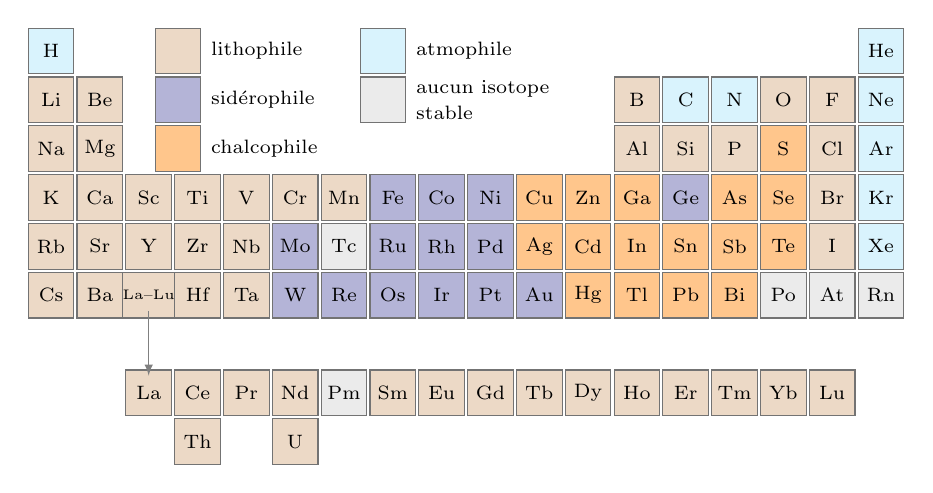
\begin{tikzpicture}[x=0.62cm, y=-0.62cm,
  lith/.style={fill=brown!30}, sid/.style={fill=blue!30!gray!45},
  chal/.style={fill=orange!45}, atm/.style={fill=cyan!15}, none/.style={fill=black!8},
  cell/.style={draw=black!55, minimum size=0.58cm, inner sep=0pt, font=\scriptsize}]
\foreach \s/\c/\r/\k in {H/1/1/atm, He/18/1/atm,
  Li/1/2/lith, Be/2/2/lith, B/13/2/lith, C/14/2/atm, N/15/2/atm, O/16/2/lith,
  F/17/2/lith, Ne/18/2/atm,
  Na/1/3/lith, Mg/2/3/lith, Al/13/3/lith, Si/14/3/lith, P/15/3/lith, S/16/3/chal,
  Cl/17/3/lith, Ar/18/3/atm,
  K/1/4/lith, Ca/2/4/lith, Sc/3/4/lith, Ti/4/4/lith, V/5/4/lith, Cr/6/4/lith,
  Mn/7/4/lith, Fe/8/4/sid, Co/9/4/sid, Ni/10/4/sid, Cu/11/4/chal, Zn/12/4/chal,
  Ga/13/4/chal, Ge/14/4/sid, As/15/4/chal, Se/16/4/chal, Br/17/4/lith, Kr/18/4/atm,
  Rb/1/5/lith, Sr/2/5/lith, Y/3/5/lith, Zr/4/5/lith, Nb/5/5/lith, Mo/6/5/sid,
  Tc/7/5/none, Ru/8/5/sid, Rh/9/5/sid, Pd/10/5/sid, Ag/11/5/chal, Cd/12/5/chal,
  In/13/5/chal, Sn/14/5/chal, Sb/15/5/chal, Te/16/5/chal, I/17/5/lith, Xe/18/5/atm,
  Cs/1/6/lith, Ba/2/6/lith, Hf/4/6/lith, Ta/5/6/lith, W/6/6/sid, Re/7/6/sid,
  Os/8/6/sid, Ir/9/6/sid, Pt/10/6/sid, Au/11/6/sid, Hg/12/6/chal, Tl/13/6/chal,
  Pb/14/6/chal, Bi/15/6/chal, Po/16/6/none, At/17/6/none, Rn/18/6/none,
  La/3/8/lith, Ce/4/8/lith, Pr/5/8/lith, Nd/6/8/lith, Pm/7/8/none, Sm/8/8/lith,
  Eu/9/8/lith, Gd/10/8/lith, Tb/11/8/lith, Dy/12/8/lith, Ho/13/8/lith,
  Er/14/8/lith, Tm/15/8/lith, Yb/16/8/lith, Lu/17/8/lith,
  Th/4/9/lith, U/6/9/lith}
  \node[cell, \k] at (\c,\r) {\s};
\node[cell, lith, minimum width=0.58cm] at (3,6) {\tiny La--Lu};
\draw[black!50, -latex] (3,6.32) -- (3,7.65);
% legend
\foreach \k/\t/\x/\y in {lith/lithophile/3.6/1, sid/sidérophile/3.6/2,
  chal/chalcophile/3.6/3, atm/atmophile/7.8/1, none/{\shortstack[l]{aucun isotope\\stable}}/7.8/2}
  \node[cell, \k, label={[font=\scriptsize]east:\t}] at (\x,\y) {};
\end{tikzpicture}
\par\smallskip{\small Les classes de Goldschmidt des éléments stables, ainsi que du thorium et de l'uranium,
dont les isotopes à longue durée de vie subsistent depuis la naissance de la Terre, colorés selon la
classe qui domine dans la Terre~; les éléments de la série des \omterm{def:b2:elements-in-the-earth:ree}{terres rares} se placent dans la case La--Lu.
Plusieurs éléments appartiennent à deux classes~: le fer, le nickel et le cobalt sont aussi lithophiles
dans le manteau oxydé~; le carbone est aussi sidérophile, le phosphore sidérophile dans les \omterm{def:b2:planet-formation-meteorites:fall-find}{météorites}.}
\end{omfigure}

\section{La Terre chondritique}

Personne ne peut échantillonner la Terre dans son ensemble~: le noyau est
hors d'atteinte, et le manteau n'atteint la surface que par morceaux. La
composition de la Terre globale se construit donc à partir de deux sources~:
les \omterm{def:b2:planet-formation-meteorites:fall-find}{météorites}, qui échantillonnent la matière dont se sont formées les
planètes, et les roches du manteau ainsi que les liquides qui en proviennent.

\begin{definition}[chondrite CI]\label{def:b2:elements-in-the-earth:ci}
Une \emph{chondrite CI}\index{chondrite CI} est un membre du groupe des \omterm{def:b2:planet-formation-meteorites:chondrule}{chondrites carbonées}
qui tire son nom de la \omterm{def:b2:planet-formation-meteorites:fall-find}{météorite} d'Ivuna~: des pierres noires et friables, faites
presque entièrement d'une matrice à grain fin, riches en minéraux hydratés et en carbone,
et presque dépourvues de \omterm{def:b2:planet-formation-meteorites:chondrule}{chondres}. Hormis l'hydrogène, le carbone, l'azote, l'oxygène
et les gaz nobles, leur composition est la plus proche de celle de la photosphère du
Soleil parmi toutes les matières connues~; elles constituent la référence de la géochimie.
\end{definition}

Le groupe compte cinq \omterm{def:b2:planet-formation-meteorites:fall-find}{météorites}, toutes des chutes~: Alais (1806), Orgueil
(1864), Tonk (1911), Ivuna (1938) et Revelstoke (1965)~; Orgueil est la
plus grande, avec quatorze kilogrammes. La composition retenue pour le groupe
est une moyenne pondérée de leurs analyses, élément par élément~; les
valeurs utilisées dans ce chapitre sont citées là où elles sont nécessaires.
% ledger: lodders:ci-table

\begin{definition}[Éléments réfractaires et volatils]
\label{def:b2:elements-in-the-earth:volatility}
Un \emph{élément réfractaire}\index{élément réfractaire} est un
élément dont la \omterm{def:b2:planet-formation-meteorites:condensation}{température de condensation} à 50 pour cent
(\cref{ch:b2:planet-formation-meteorites}) est supérieure à celles du magnésium,
du silicium et du fer, \qtyrange{1310}{1340}{K} à \qty{e-4}{bar}~;
un \emph{élément volatil}\index{élément volatil} est un élément
dont la \omterm{def:b2:planet-formation-meteorites:condensation}{température de condensation} est inférieure à celles-ci.
\end{definition}

Le magnésium sert d'étalon. Le magnésium est lithophile~: il se condense avec l'essentiel
de la roche et n'entre pas dans le noyau~; le rapport d'un élément au magnésium
dans la Terre silicatée, divisé par le même rapport dans les \omterm{def:b2:elements-in-the-earth:ci}{chondrites CI}, mesure la
part de cet élément que la Terre silicatée a conservée par rapport à une matière de
départ chondritique. L'eau, le carbone et les autres composés volatils que contiennent
les \omterm{def:b2:elements-in-the-earth:ci}{chondrites CI}, et que la Terre n'a pas conservés, s'annulent dans le rapport.

\begin{definition}[Terre silicatée globale, manteau primitif]
\label{def:b2:elements-in-the-earth:bse}
La \emph{Terre silicatée globale}\index{Terre silicatée globale} est la
Terre privée de son noyau~: manteau, croûte, océan et atmosphère pris ensemble,
comme s'ils étaient mélangés. La même composition porte le nom de
\emph{manteau primitif}\index{manteau primitif}~: le manteau tel qu'il était
après la formation du noyau et avant qu'une croûte n'en ait été extraite.
\end{definition}

Les estimations du \omterm{def:b2:elements-in-the-earth:bse}{manteau primitif} reposent sur les roches du manteau ayant perdu le moins
de liquide, les péridotites remontées en xénolites dans les laves (photographie ci-dessous)
ou affleurant dans les chaînes de montagnes, et sur l'hypothèse que les \omterm{def:b2:elements-in-the-earth:goldschmidt}{éléments
lithophiles} réfractaires sont dans les proportions chondritiques les uns par rapport aux autres.
Un résultat largement utilisé, avec 22.8 pour cent de magnésium, 21.0 pour cent de silicium
et 6.26 pour cent de fer en masse, figure dans le tableau des compositions plus loin.
% ledger: ms95:pm-trace, ms95:pm-oxides

\begin{omfigure}
\centering
\begin{minipage}{0.48\linewidth}
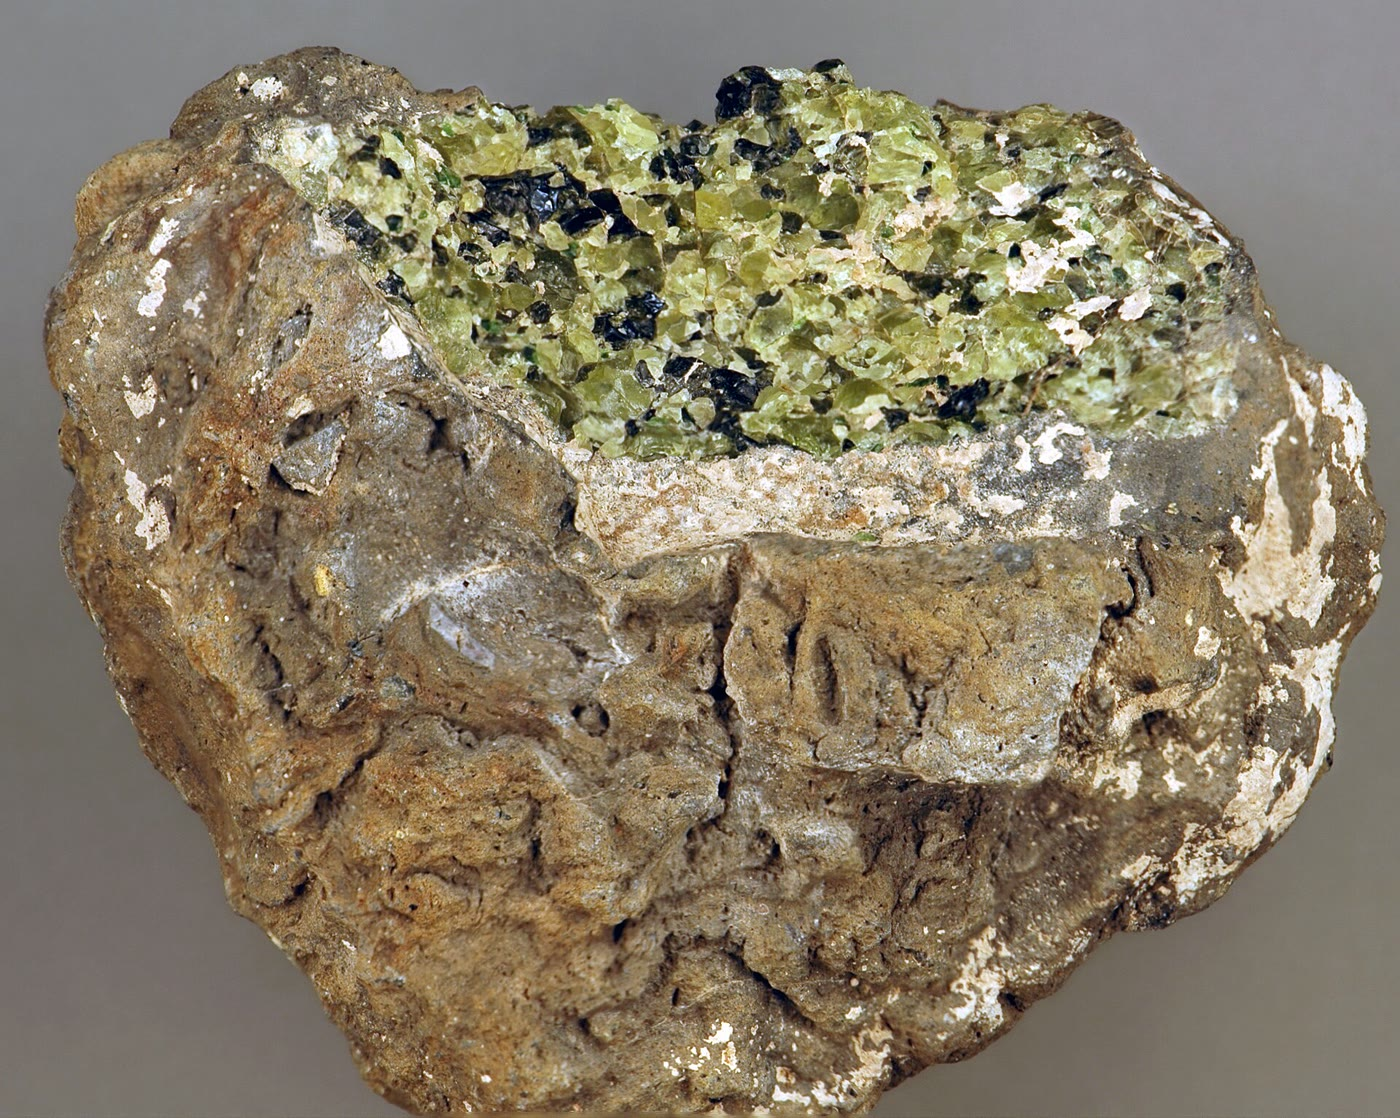
\includegraphics[width=\linewidth]{images/book4/b2-lherzolite-xenolith.jpg}
\end{minipage}\hfill
\begin{minipage}{0.48\linewidth}
{\small Nodule de péridotite du manteau (lherzolite) dans une lave basaltique
de Kilbourne Hole, Nouveau-Mexique, large de \qty{7.4}{cm} dans sa plus grande
dimension~: olivine jaune-vert et pyroxène sombre. La lave l'a arrachée au
manteau supérieur et l'a portée jusqu'à la surface. James St.~John, CC BY 2.0.}
\end{minipage}
\end{omfigure}

La figure ci-dessous compare cette Terre silicatée aux \omterm{def:b2:elements-in-the-earth:ci}{chondrites CI}, élément par élément,
en fonction de la \omterm{def:b2:planet-formation-meteorites:condensation}{température de condensation} du chapitre précédent. Elle classe les
éléments d'une manière qu'aucune autre observation ne permet. Les \omterm{def:b2:elements-in-the-earth:goldschmidt}{éléments lithophiles}
réfractaires, du zirconium et des \omterm{def:b2:elements-in-the-earth:ree}{terres rares} jusqu'au strontium et au baryum, se placent
tous au même niveau, à vingt pour cent près les uns des autres~: la Terre silicatée
les a tous conservés dans leurs proportions chondritiques. Les \omterm{def:b2:elements-in-the-earth:goldschmidt}{éléments lithophiles}
volatils s'effondrent avec leur \omterm{def:b2:planet-formation-meteorites:condensation}{température de condensation}~: environ un cinquième du potassium
et du sodium, un dixième du rubidium, un centième du chlore et quelques millièmes
du brome et de l'iode s'y trouvent. Les \omterm{def:b2:elements-in-the-earth:goldschmidt}{éléments sidérophiles} se situent très en dessous
de tous les \omterm{def:b2:elements-in-the-earth:goldschmidt}{éléments lithophiles} de même volatilité~: la Terre silicatée contient un
septième de sa part de fer, un treizième du nickel et environ trois millièmes des métaux
du groupe du platine et de l'or. Ces éléments sont passés dans le noyau. Les \omterm{def:b2:elements-in-the-earth:goldschmidt}{éléments
chalcophiles}, pour la plupart également volatils, sont appauvris selon les deux critères.

\begin{omfigure}
\centering
\begin{tikzpicture}
\begin{axis}[omrecord, width=0.95\linewidth, height=8.2cm, ymode=log,
  xmin=500, xmax=1800, ymin=8e-4, ymax=3, x dir=reverse,
  xlabel={température de condensation à 50 pour cent, à \qty{e-4}{bar} (K)},
  ylabel={$(X/\mathrm{Mg})_{\mathrm{BSE}}\,/\,(X/\mathrm{Mg})_{\mathrm{CI}}$},
  legend pos=south west, legend cell align=left, legend style={font=\scriptsize},
  tick label style={font=\scriptsize}, label style={font=\small},
  scaled x ticks=false, xticklabel style={/pgf/number format/1000 sep={}}]
\addplot[black!40, dashed, domain=500:1800, samples=2, forget plot] {1};
\addplot[only marks, mark=*, mark size=1.6pt, brown!70!black]
  table[x=T, y=ratio] {figdata/out/bachelor-2-geochem-volat-lith.dat};
\addlegendentry{lithophile}
\addplot[only marks, mark=square*, mark size=1.6pt, blue!60!black]
  table[x=T, y=ratio] {figdata/out/bachelor-2-geochem-volat-sid.dat};
\addlegendentry{sidérophile}
\addplot[only marks, mark=triangle*, mark size=2pt, orange!80!black]
  table[x=T, y=ratio] {figdata/out/bachelor-2-geochem-volat-chal.dat};
\addlegendentry{chalcophile}
\node[font=\tiny, brown!50!black, anchor=south] at (axis cs:1600,1.35)
  {Zr, Hf, Al, Sc, Y, Th, U, Ti, Ca, Sr, Ba, terres rares};
\begin{scope}[font=\tiny, brown!50!black]
\node[anchor=west] at (axis cs:1328,1.0) {Mg};
\node[anchor=north] at (axis cs:1310,0.80) {Si};
\node[anchor=west] at (axis cs:1150,0.23) {Mn};
\node[anchor=south] at (axis cs:1142,0.47) {Li};
\node[anchor=south] at (axis cs:1010,0.195) {K};
\node[anchor=north] at (axis cs:958,0.22) {Na};
\node[anchor=north] at (axis cs:908,0.175) {B};
\node[anchor=north] at (axis cs:800,0.116) {Rb};
\node[anchor=south] at (axis cs:734,0.175) {F};
\node[anchor=west] at (axis cs:795,0.0477) {Cs};
\node[anchor=west] at (axis cs:944,0.0102) {Cl};
\node[anchor=north] at (axis cs:546,0.0061) {Br};
\node[anchor=south] at (axis cs:535,0.0088) {I};
\end{scope}
\begin{scope}[font=\tiny, blue!50!black]
\node[anchor=west] at (axis cs:1325,0.144) {Fe};
\node[anchor=east] at (axis cs:1364,0.0775) {Ni};
\node[anchor=west] at (axis cs:1342,0.088) {Co};
\node[anchor=west] at (axis cs:1780,0.137) {W};
\node[anchor=south] at (axis cs:1590,0.0206) {Mo};
\node[anchor=north] at (axis cs:883,0.0139) {Ge};
\node[anchor=north] at (axis cs:1500,0.0026) {Re, Os, Ir, Ru, Pt, Pd};
\node[anchor=north] at (axis cs:1060,0.0026) {Au};
\end{scope}
\begin{scope}[font=\tiny, orange!60!black]
\node[anchor=west] at (axis cs:1030,0.0993) {Cu};
\node[anchor=north] at (axis cs:996,0.0167) {Ag};
\node[anchor=south] at (axis cs:726,0.0746) {Zn};
\node[anchor=south] at (axis cs:704,0.0325) {Sn};
\node[anchor=east] at (axis cs:735,0.0246) {Pb};
\node[anchor=west] at (axis cs:648,0.0249) {Cd};
\node[anchor=east] at (axis cs:715,0.0022) {Te};
\node[anchor=north] at (axis cs:690,0.0016) {Se};
\node[anchor=west] at (axis cs:660,0.0019) {S};
\end{scope}
\end{axis}
\end{tikzpicture}
\par\smallskip{\small La Terre silicatée comparée aux \omterm{def:b2:elements-in-the-earth:ci}{chondrites CI}~: pour chaque élément
$X$, le rapport $X/\mathrm{Mg}$ dans la \omterm{def:b2:elements-in-the-earth:bse}{Terre silicatée globale}, divisé par le même
rapport dans les \omterm{def:b2:elements-in-the-earth:ci}{chondrites CI}, en fonction de la \omterm{def:b2:planet-formation-meteorites:condensation}{température de condensation} à 50 pour
cent (les plus chaudes à gauche). Les \omterm{def:b2:elements-in-the-earth:goldschmidt}{éléments lithophiles} réfractaires sont chondritiques
les uns par rapport aux autres~; les \omterm{def:b2:elements-in-the-earth:volatility}{éléments volatils} sont d'autant plus appauvris
que leur \omterm{def:b2:planet-formation-meteorites:condensation}{température de condensation} est basse~; les \omterm{def:b2:elements-in-the-earth:goldschmidt}{éléments sidérophiles} et
chalcophiles le sont bien davantage. Données~: McDonough et Sun (1995)~; Lodders (2003).}
\end{omfigure}
% ledger: ms95:pm-trace, lodders:ci-table, lodders:tc-table, lodders:tc-more

Les \omterm{def:b2:elements-in-the-earth:goldschmidt}{éléments lithophiles} réfractaires se situent environ 15 pour cent au-dessus du magnésium.
Les deux ne peuvent pas être exactement chondritiques~: soit la Terre a gagné des \omterm{def:b2:elements-in-the-earth:volatility}{éléments
réfractaires}, soit elle a perdu un peu de magnésium, soit le magnésium du modèle est sous-estimé
(\cref{exo:b2:elements-in-the-earth:12}). Le silicium, à 0.83, reste nettement en deçà du niveau
réfractaire~; une partie du silicium manquant se trouve peut-être dans le noyau (problème).

Les \omterm{def:b2:elements-in-the-earth:goldschmidt}{éléments sidérophiles} de la Terre silicatée, combinés à une Terre globale
chondritique, permettent de peser le noyau. Supposons que la Terre globale ait
le rapport CI $r_X = X/\mathrm{Mg}$ pour un \omterm{def:b2:elements-in-the-earth:goldschmidt}{élément sidérophile} $X$, et que
le noyau contienne la concentration $c_X$ de cet élément mais aucun magnésium.

\begin{proposition}[Fraction massique du noyau à partir d'un rapport chondritique]
\label{prop:b2:elements-in-the-earth:core}
Soit $x$ la fraction massique du noyau, $C_X$ et $C_{\mathrm{Mg}}$ les
concentrations de $X$ et du magnésium dans la Terre silicatée, et $c_X$ celle
de $X$ dans le noyau. Si la Terre a le rapport chondritique $r_X$, alors
\[
  \frac{x}{1-x} = \frac{r_X C_{\mathrm{Mg}} - C_X}{c_X}.
\]
\end{proposition}

\begin{proof}
Une masse $M$ de Terre contient $(1-x)MC_X + xMc_X$ de
$X$ et $(1-x)MC_{\mathrm{Mg}}$ de magnésium. Leur rapport
vaut $r_X$~: $(1-x)C_X + xc_X = r_X(1-x)C_{\mathrm{Mg}}$.
En divisant par $(1-x)c_X$, on obtient le résultat.
\end{proof}

Pour le fer, $r_{\mathrm{Fe}} = \num{182800}/\num{95870} = 1.907$ dans les \omterm{def:b2:elements-in-the-earth:ci}{chondrites
CI}, 22.8 pour cent de magnésium et 6.26 pour cent de fer dans la Terre silicatée, et 85.5
pour cent de fer dans un noyau modèle~: la proposition donne $x/(1-x) = 0.435$, soit
un noyau représentant 30 pour cent de la masse de la Terre. La sismologie, en intégrant
la masse volumique du modèle de Terre de référence, donne 32.5 pour cent. L'accord, à
un dixième près, conforte l'image d'une Terre chondritique dont le fer est surtout dans
le noyau~; l'écart mesure de combien le rapport fer/magnésium de la Terre s'écarte du
rapport chondritique (problème). Le même bilan indique où se trouve chaque élément de
la Terre (figure ci-dessous)~: presque tout son platine, son iridium et son or, ainsi
que la plus grande part de son fer, de son nickel et de son soufre, sont dans le noyau.
% ledger: lodders:ci-table, ms95:pm-trace, mcd03:core, data:prem

\begin{omfigure}
\centering
\begin{tikzpicture}
\begin{axis}[omrecord, xbar, width=0.8\linewidth, height=6.4cm, bar width=5pt,
  xmin=0, xmax=100, ymin=0.4, ymax=14.6, y dir=reverse,
  ytick={1,...,14}, yticklabels from table={figdata/out/bachelor-2-geochem-budget.dat}{el},
  xlabel={part de l'inventaire terrestre contenu dans le noyau (pour cent)},
  tick label style={font=\scriptsize}, label style={font=\small},
  nodes near coords, nodes near coords align={horizontal},
  every node near coord/.append style={font=\tiny, /pgf/number format/fixed,
    /pgf/number format/precision=1}]
\addplot[fill=blue!35!gray!50, draw=black!60]
  table[x=share, y=idx] {figdata/out/bachelor-2-geochem-budget.dat};
\end{axis}
\end{tikzpicture}
\par\smallskip{\small Où se trouvent les éléments de la Terre~: la part de chaque
élément retenue dans le noyau, d'après une composition modèle du noyau, le
\omterm{def:b2:elements-in-the-earth:bse}{manteau primitif} et un noyau de 32.5 pour cent de la masse de la Terre. Données~:
McDonough (2003)~; McDonough et Sun (1995)~; modèle de Terre de référence.}
\end{omfigure}
% ledger: mcd03:core, ms95:pm-trace, data:prem

\section{Manteau et croûtes}

Depuis sa formation, la Terre silicatée s'est divisée en un manteau et deux sortes
de croûte. La croûte océanique naît de la fusion du manteau sous les dorsales
océaniques~; la croûte continentale résulte d'une longue histoire de fusion au-dessus
des zones de subduction, de remaniement et d'érosion (chapitres ultérieurs).
Deux liquides de référence issus du manteau servent de repères à la discussion.

\begin{definition}[Basalte de dorsale, basalte d'île océanique]
\label{def:b2:elements-in-the-earth:morb-oib}
Un \emph{basalte de dorsale}\index{basalte de dorsale} (MORB) est un basalte
émis à une dorsale océanique, roche du sommet de la croûte océanique. Un
\emph{basalte d'île océanique}\index{basalte d'île océanique} (OIB) est un basalte émis
par un volcan océanique loin des limites de plaques, comme ceux d'Hawaï, que
l'on attribue en général à un panache mantellique (volume de première année).
\end{definition}

Le MORB moyen du tableau ci-dessous est une moyenne mondiale établie à partir de
771 segments de dorsale, chacun pondéré par sa longueur et par sa vitesse d'expansion,
de sorte que la moyenne représente la croûte que produisent les dorsales.
La colonne OIB correspond à une roche unique~: le basalte de référence BHVO-2,
prélevé en 1995 dans une coulée qui a débordé du cratère Halemaumau du Kilauea, à
Hawaï, en 1919, et analysé par de nombreux laboratoires, si bien que la plupart
de ses \omterm{def:b2:elements-in-the-earth:ree}{terres rares} sont connues à un pour cent près. La croûte continentale
supérieure est une moyenne estimée à partir des roches de surface et des sédiments.
% ledger: gale13:allmorb, usgs:bhvo2-origin, usgs:bhvo2-major, rg14:crust

\begin{table}[h]
\centering
\small
\begin{tabular}{lrrrr}
\hline
oxyde (\% massique) & \omterm{def:b2:elements-in-the-earth:bse}{manteau primitif} & MORB & OIB (BHVO-2) & croûte cont.\ sup.\\
\hline
\ce{SiO2} & 45.0 & 50.47 & 49.60 & 66.6\\
\ce{TiO2} & 0.201 & 1.68 & 2.731 & 0.64\\
\ce{Al2O3} & 4.45 & 14.70 & 13.44 & 15.4\\
FeO (total) & 8.05 & 10.43 & 11.15 & 5.04\\
MnO & 0.135 & 0.184 & 0.1690 & 0.10\\
MgO & 37.8 & 7.58 & 7.257 & 2.48\\
CaO & 3.55 & 11.39 & 11.40 & 3.59\\
\ce{Na2O} & 0.36 & 2.79 & 2.219 & 3.27\\
\ce{K2O} & 0.029 & 0.160 & 0.5130 & 2.80\\
\ce{P2O5} & 0.021 & 0.184 & 0.2685 & 0.15\\
\hline
\end{tabular}
\caption{Compositions en éléments majeurs de quatre réservoirs. Le BHVO-2 donne son fer sous
\ce{Fe2O3} (12.39 pour cent), ici converti en FeO. Données~: McDonough et Sun
(1995)~; Gale et al. (2013)~; fiche d'information USGS sur le BHVO-2~; Rudnick et
Gao (2014).}
\label{tab:b2:elements-in-the-earth:majors}
\end{table}
% ledger: ms95:pm-oxides, gale13:allmorb, usgs:bhvo2-major, rg14:crust

En parcourant le tableau, on lit l'histoire de la fusion. Le manteau est une péridotite
riche en magnésium, avec près de 38 pour cent de MgO et moins de 5 pour cent de \ce{Al2O3}
et de CaO. Ses liquides, les basaltes, contiennent cinq fois moins de magnésium et
trois fois plus de calcium et d'aluminium~: les éléments qui entrent facilement dans le
liquide quittent le manteau en premier. Le potassium, le sodium et le titane sont encore
plus riches dans les liquides que dans le manteau, et le potassium est le plus riche de
tous dans la croûte continentale, presque cent fois sa concentration dans le \omterm{def:b2:elements-in-the-earth:bse}{manteau
primitif}. Le silicium ne passe que peu du manteau aux basaltes, et beaucoup plus dans la
croûte continentale, dont la composition moyenne est proche de celle d'une granodiorite.

\section{Éléments en traces}

Dix oxydes constituent environ 99 pour cent de chaque roche du tableau
ci-dessus. Les autres éléments, présents en parties par million, suivent les mêmes
processus que les éléments majeurs, mais y sont beaucoup plus sensibles.

\begin{definition}[Élément en traces]\label{def:b2:elements-in-the-earth:trace}
Un \emph{élément en traces}\index{élément en traces} d'une roche est un élément dont
la concentration est conventionnellement inférieure à 0.1 pour cent en masse
(\qty{1000}{ppm}). Les éléments en traces forment rarement des minéraux qui leur soient propres~;
ils se substituent aux éléments majeurs dans les sites des réseaux cristallins.
\end{definition}

Un \omterm{def:b2:elements-in-the-earth:trace}{élément en traces} est si dilué que sa propre concentration ne modifie
ni les cristaux ni le liquide~: sa répartition entre eux est alors un
simple rapport, indépendant de sa concentration sur une large gamme.

\begin{definition}[Coefficient de partage minéral--liquide~; éléments compatibles et
incompatibles]\label{def:b2:elements-in-the-earth:partition}
Le \emph{coefficient de partage minéral--liquide}\index{coefficient de partage minéral--liquide}
d'un élément dans un minéral est le rapport de ses concentrations
dans le minéral et dans un liquide silicaté en équilibre avec lui,
$D = C_{\mathrm{mineral}}/C_{\mathrm{melt}}$. Pour une roche composée de plusieurs minéraux de
fractions massiques $x_i$, le \emph{coefficient de partage global} est
$\bar D = C_{\mathrm{rock}}/C_{\mathrm{melt}}$. Dans une roche, un
\emph{élément compatible}\index{élément compatible} est un élément tel que $\bar D > 1$, et un
\emph{élément incompatible}\index{élément incompatible} un élément tel que $\bar D < 1$.
\end{definition}

\begin{proposition}[Coefficient de partage global]
\label{prop:b2:elements-in-the-earth:bulk-d}
Si chaque minéral de la roche est en équilibre avec le même liquide, le
coefficient de partage global est la moyenne des coefficients des
minéraux, pondérée par les fractions massiques~: $\bar D = \sum_i x_i D_i$.
\end{proposition}

\begin{proof}
La roche contient $C_{\mathrm{rock}} = \sum_i x_i C_i$, et chaque minéral
$C_i = D_i C_{\mathrm{melt}}$. En divisant par $C_{\mathrm{melt}}$, on obtient le résultat.
\end{proof}

Qu'un ion s'insère dans un site dépend de son rayon et de sa charge. Un ion
proche en rayon et en charge de l'ion majeur d'un site, comme \ce{Ni^2+} pour
\ce{Mg^2+} dans l'olivine, y entre facilement et est compatible. Un ion
beaucoup plus gros, comme \ce{Rb+} ou \ce{Ba^2+}, ou plus fortement chargé, comme
\ce{Zr^4+} ou \ce{Nb^5+}, déforme le réseau et est rejeté dans le liquide~:
il est incompatible dans les minéraux du manteau. Deux groupes d'\omterm{def:b2:elements-in-the-earth:partition}{éléments
incompatibles} se comportent différemment plus tard, lorsque l'eau intervient.

\begin{definition}[Éléments lithophiles à grand rayon ionique et à fort champ électrostatique]
\label{def:b2:elements-in-the-earth:lile-hfse}
Les \emph{éléments lithophiles à grand rayon ionique}\index{élément lithophile à grand rayon ionique}
(LILE) sont des \omterm{def:b2:elements-in-the-earth:partition}{éléments incompatibles} dont les ions sont grands
et de faible charge, $+1$ ou $+2$~: potassium, rubidium, césium, strontium,
baryum. Les \emph{éléments à fort champ électrostatique}\index{élément à fort champ électrostatique}
(HFSE) sont des \omterm{def:b2:elements-in-the-earth:partition}{éléments incompatibles} dont les ions sont petits
et fortement chargés, $+4$ ou $+5$~: zirconium, hafnium, niobium, tantale, titane.
\end{definition}

Les LILE se dissolvent facilement dans les fluides riches en eau, les HFSE presque
pas. Une roche altérée par l'eau, ou un liquide ayant hérité de fluides, comme
au-dessus des zones de subduction, transporte donc des LILE avec peu de HFSE.

\begin{definition}[Terre rare]\label{def:b2:elements-in-the-earth:ree}
Les \emph{terres rares}\index{terre rare} (REE) sont les quinze
lanthanides, du lanthane au lutécium~; le prométhium n'a pas d'isotope
stable. Tous sont lithophiles et réfractaires, presque tous trivalents,
et leur rayon ionique diminue régulièrement du lanthane au lutécium~;
l'europium peut aussi être divalent dans les liquides réduits.
\end{definition}

Parce que les \omterm{def:b2:elements-in-the-earth:ree}{terres rares} ne diffèrent régulièrement que par leur rayon, elles se
fractionnent régulièrement~: les plus légères, du lanthane au samarium, sont les moins
compatibles~; les plus lourdes, du gadolinium au lutécium, s'insèrent mieux dans
certains minéraux, surtout le grenat (figure ci-dessous). Dans une roche qui contient
du grenat, les \omterm{def:b2:elements-in-the-earth:ree}{terres rares} lourdes deviennent compatibles~: un liquide issu d'une
telle roche est riche en \omterm{def:b2:elements-in-the-earth:ree}{terres rares} légères et pauvre en \omterm{def:b2:elements-in-the-earth:ree}{terres rares} lourdes.

\begin{omfigure}
\centering
\begin{tikzpicture}
\begin{axis}[omrecord, width=0.78\linewidth, height=6.4cm, ymode=log,
  xmin=0.6, xmax=9.4, ymin=5e-4, ymax=20,
  xtick={1,...,9}, xticklabels from table={figdata/out/bachelor-2-geochem-dvals.dat}{el},
  ylabel={coefficient de partage $D$}, legend pos=south east,
  legend cell align=left, legend style={font=\scriptsize},
  tick label style={font=\scriptsize}, label style={font=\small}]
\addplot[black!40, dashed, domain=0.6:9.4, samples=2, forget plot] {1};
\addplot[thick, green!45!black, mark=*] table[x=idx, y=cpx] {figdata/out/bachelor-2-geochem-dvals.dat};
\addlegendentry{clinopyroxène}
\addplot[thick, red!70!black, mark=square*] table[x=idx, y=gar] {figdata/out/bachelor-2-geochem-dvals.dat};
\addlegendentry{grenat}
\addplot[thick, olive!70!black, mark=triangle*] table[x=idx, y=ol] {figdata/out/bachelor-2-geochem-dvals.dat};
\addlegendentry{olivine + orthopyroxène + spinelle}
\addplot[very thick, black, mark=diamond*] table[x=idx, y=bulk] {figdata/out/bachelor-2-geochem-dvals.dat};
\addlegendentry{roche totale (65/18/17 pour cent)}
\node[font=\scriptsize, anchor=south west] at (axis cs:0.7,1) {compatible};
\node[font=\scriptsize, anchor=north west] at (axis cs:0.7,1) {incompatible};
\end{axis}
\end{tikzpicture}
\par\smallskip{\small \omterm{def:b2:elements-in-the-earth:partition}{Coefficients de partage minéral--liquide} des \omterm{def:b2:elements-in-the-earth:ree}{terres rares} pour
le clinopyroxène, le grenat et un mélange d'olivine, d'orthopyroxène et de spinelle,
et coefficient global d'une pyroxénite à grenat de 65 pour cent de clinopyroxène,
18 pour cent de grenat et 17 pour cent des autres minéraux (proposition ci-dessus).
Le grenat rend les \omterm{def:b2:elements-in-the-earth:ree}{terres rares} lourdes compatibles. Données~: Budahn (1991).}
\end{omfigure}
% ledger: budahn91:d-ree, budahn91:modes

\section{Diagrammes normalisés}

Les abondances d'éléments voisins diffèrent par des facteurs importants à cause de l'histoire
nucléaire de la matière~: les éléments de numéro atomique pair sont plus abondants que
leurs voisins impairs, comme le montre la colonne CI des \omterm{def:b2:elements-in-the-earth:ree}{terres rares} (lanthane 0.232, cérium
0.621, praséodyme 0.0928 ppm). Tracées brutes, les \omterm{def:b2:elements-in-the-earth:ree}{terres rares} d'une roche forment une dent
de scie qui masque son histoire géologique. Diviser par une référence supprime cet effet.
% ledger: lodders:ci-table

\begin{definition}[Diagramme normalisé]\label{def:b2:elements-in-the-earth:normalised}
Un \emph{diagramme normalisé}\index{diagramme normalisé} porte, pour une série d'éléments
dans un ordre fixé, la concentration d'un échantillon divisée par celle d'une référence,
$X_N = C_X/C_X^{\mathrm{ref}}$, sur une échelle logarithmique. Les \omterm{def:b2:elements-in-the-earth:ree}{terres rares} sont
normalisées aux \omterm{def:b2:elements-in-the-earth:ci}{chondrites CI} dans l'ordre des numéros atomiques~; un ensemble plus
long d'\omterm{def:b2:elements-in-the-earth:partition}{éléments incompatibles}, souvent appelé diagramme en araignée, est normalisé au
\omterm{def:b2:elements-in-the-earth:bse}{manteau primitif} et ordonné par incompatibilité décroissante lors de la fusion du manteau.
\end{definition}

Un échantillon de mêmes proportions que la référence se trace en ligne
horizontale~; sa hauteur donne l'enrichissement. Une pente traduit un fractionnement
entre éléments légers et lourds, mesuré par un rapport tel que
$(\mathrm{La}/\mathrm{Yb})_N$. Un élément isolé hors de la ligne est une anomalie.

\begin{proposition}[Anomalie en europium]\label{prop:b2:elements-in-the-earth:normalised}
Sur un \omterm{def:b2:elements-in-the-earth:normalised}{diagramme normalisé} où le motif est une droite en $\log X_N$ entre
le samarium et le gadolinium, la valeur attendue pour l'europium, qui
se situe à mi-chemin, est $\mathrm{Eu}^* = \sqrt{\mathrm{Sm}_N\,\mathrm{Gd}_N}$.
L'\emph{anomalie en europium}\index{anomalie en europium} est
$\mathrm{Eu}/\mathrm{Eu}^* = \mathrm{Eu}_N/\sqrt{\mathrm{Sm}_N\,\mathrm{Gd}_N}$~:
inférieure à 1, elle est négative~; supérieure à 1, positive.
\end{proposition}

\begin{proof}
Samarium, europium et gadolinium sont consécutifs, à pas égaux le long
de l'axe. Une droite en $\log X_N$ prend au point médian la moyenne des
valeurs extrêmes~: $\log \mathrm{Eu}^* = \tfrac12(\log \mathrm{Sm}_N + \log \mathrm{Gd}_N)$,
soit le logarithme de la moyenne géométrique.
\end{proof}

L'europium est la seule \omterm{def:b2:elements-in-the-earth:ree}{terre rare} qui puisse être divalente. \ce{Eu^2+} a presque le rayon
de \ce{Ca^2+} et de \ce{Sr^2+}~: le feldspath plagioclase l'accueille donc là où il rejette
les \omterm{def:b2:elements-in-the-earth:ree}{terres rares} trivalentes. Un liquide duquel a cristallisé du plagioclase présente une
anomalie négative~; la roche riche en plagioclase qui reste en arrière, une anomalie positive.

\begin{omfigure}
\centering
\begin{tikzpicture}
\begin{axis}[omrecord, width=0.8\linewidth, height=6.4cm, ymode=log,
  xmin=0.6, xmax=13.4, ymin=5, ymax=250,
  xtick={1,...,13}, xticklabels from table={figdata/out/bachelor-2-geochem-ree.dat}{el},
  ylabel={échantillon / chondrite CI}, legend pos=north east, legend cell align=left,
  legend style={font=\scriptsize}, tick label style={font=\scriptsize},
  label style={font=\small}]
\addplot[thick, blue!70!black, mark=*] table[x=idx, y=morb] {figdata/out/bachelor-2-geochem-ree.dat};
\addlegendentry{MORB moyen}
\addplot[thick, red!70!black, mark=square*] table[x=idx, y=oib] {figdata/out/bachelor-2-geochem-ree.dat};
\addlegendentry{OIB (BHVO-2, Hawaï)}
\addplot[thick, brown!70!black, mark=triangle*] table[x=idx, y=ucc] {figdata/out/bachelor-2-geochem-ree.dat};
\addlegendentry{croûte continentale supérieure}
\end{axis}
\end{tikzpicture}
\par\smallskip{\small Motifs des \omterm{def:b2:elements-in-the-earth:ree}{terres rares} normalisés aux \omterm{def:b2:elements-in-the-earth:ci}{chondrites CI} (le
thulium est omis, faute de valeur pour le MORB). Le MORB moyen est plat, légèrement
plus pauvre en \omterm{def:b2:elements-in-the-earth:ree}{terres rares} légères~; le basalte hawaïen en est enrichi~; la
croûte supérieure l'est fortement, avec une anomalie négative en europium. Données~:
Gale et al. (2013)~; fiche USGS du BHVO-2~; Rudnick et Gao~; Lodders (2003).}
\end{omfigure}
% ledger: gale13:allmorb, usgs:bhvo2-trace, rg03:ucc-trace, lodders:ci-table

Les trois motifs de la figure ci-dessus se lisent comme trois histoires. Le MORB moyen se situe
environ 25 fois au-dessus de la \omterm{def:b2:planet-formation-meteorites:chondrule}{chondrite}, presque plat, avec $(\mathrm{La}/\mathrm{Sm})_N
= 0.85$~: sa source mantellique avait déjà perdu une partie de ses éléments les plus incompatibles
au profit de fusions antérieures, dont celle qui a produit
la croûte continentale. Le basalte hawaïen
est enrichi en \omterm{def:b2:elements-in-the-earth:ree}{terres rares} légères, $(\mathrm{La}/\mathrm{Yb})_N = 5.4$, et ses \omterm{def:b2:elements-in-the-earth:ree}{terres rares}
lourdes sont plus basses que celles du MORB~: il provient d'un degré de fusion plus faible,
au cours duquel le grenat a retenu les lourdes. La croûte continentale supérieure est
enrichie plus de cent fois en lanthane, avec $(\mathrm{La}/\mathrm{Yb})_N = 10.9$ et
$\mathrm{Eu}/\mathrm{Eu}^* = 0.72$~: c'est le produit de fusions répétées, et son déficit
en europium est compatible avec du plagioclase resté dans la croûte profonde.

\begin{omfigure}
\centering
\begin{tikzpicture}
\begin{axis}[omrecord, width=\linewidth, height=6.6cm, ymode=log,
  xmin=0.5, xmax=27.5, ymin=1, ymax=400,
  xtick={1,...,27}, xticklabels from table={figdata/out/bachelor-2-geochem-spider.dat}{el},
  ylabel={échantillon / manteau primitif}, legend pos=north east, legend cell align=left,
  legend style={font=\scriptsize}, tick label style={font=\scriptsize},
  label style={font=\small}]
\addplot[thick, blue!70!black, mark=*, mark size=1.4pt] table[x=idx, y=morb] {figdata/out/bachelor-2-geochem-spider.dat};
\addlegendentry{MORB moyen}
\addplot[thick, red!70!black, mark=square*, mark size=1.4pt] table[x=idx, y=oib] {figdata/out/bachelor-2-geochem-spider.dat};
\addlegendentry{OIB (BHVO-2)}
\addplot[thick, brown!70!black, mark=triangle*, mark size=1.6pt] table[x=idx, y=ucc] {figdata/out/bachelor-2-geochem-spider.dat};
\addlegendentry{croûte continentale supérieure}
\end{axis}
\end{tikzpicture}
\par\smallskip{\small \omterm{def:b2:elements-in-the-earth:partition}{Éléments incompatibles} normalisés au \omterm{def:b2:elements-in-the-earth:bse}{manteau primitif}, du plus
incompatible à gauche. La croûte continentale montre les LILE élevés, des creux
profonds au niveau du niobium, du tantale et du titane, et le pic de plomb hérité
de la fusion au-dessus des zones de subduction~; le basalte hawaïen montre une bosse
au niveau du niobium et du tantale. Potassium et titane calculés à partir des
oxydes. Données~: comme pour la figure des \omterm{def:b2:elements-in-the-earth:ree}{terres rares}~; McDonough et Sun (1995).}
\end{omfigure}
% ledger: gale13:allmorb, usgs:bhvo2-trace, usgs:bhvo2-major, rg03:ucc-trace, ms95:pm-trace

Le diagramme en araignée ci-dessus accentue le contraste. Dans la croûte continentale, le niobium et le tantale
se situent bien en dessous de leurs voisins, le thorium et le lanthane, le titane en dessous des siens, et le plomb nettement au-dessus~: $(\mathrm{Nb}/\mathrm{La})_N =
0.38$. Dans le basalte hawaïen, ce même rapport vaut 1.17, et 0.99 dans le MORB moyen.
Le motif de la croûte est la signature des liquides formés
au-dessus des zones de subduction, où des fluides ont transporté
les LILE et le plomb dans le coin de manteau et ont laissé derrière eux les HFSE (chapitres ultérieurs)~; les \omterm{def:b2:elements-in-the-earth:morb-oib}{basaltes d'île océanique} n'en présentent pas.
Le diagramme en araignée d'un seul échantillon
peut donc distinguer une lave d'arc d'une lave d'île océanique,
ou révéler un basalte contaminé par de la croûte continentale (\cref{exo:b2:elements-in-the-earth:11}).

\begin{inthelab}[D'une roche à une liste d'éléments en traces]
\begin{minipage}[t]{0.6\linewidth}
\vspace{0pt}
Un géochimiste qui veut obtenir les \omterm{def:b2:elements-in-the-earth:trace}{éléments en traces} d'un basalte part de quelques
centaines de grammes de son cœur le plus frais, exempt de croûte altérée et de
veines. La roche est concassée, puis broyée en poudre fine dans un broyeur dont le
matériau ne contaminera pas les éléments étudiés. Une petite portion de la poudre est
mise en solution dans des acides, ou fondue avec un fondant, et la solution est
analysée par spectrométrie de masse à plasma à couplage inductif, qui mesure la plupart
des éléments du diagramme en araignée à la fois. Avec chaque lot d'échantillons,
le laboratoire analyse des matériaux de référence de composition connue, comme le
basalte hawaïen BHVO-2~: ses valeurs proviennent d'une étude qui a combiné les moyennes
de nombreux laboratoires, 132 pour le lanthane, et certaines d'entre elles, comme
celles du néodyme et du samarium, par dilution isotopique, qui compte les atomes
d'un élément par rapport à une quantité connue ajoutée d'un de ses isotopes. Si le
résultat du laboratoire pour le matériau de référence se situe dans l'incertitude de
la valeur admise, les résultats des échantillons inconnus sont acceptés avec lui.
\end{minipage}\hfill
\begin{minipage}[t]{0.36\linewidth}
\vspace{0pt}
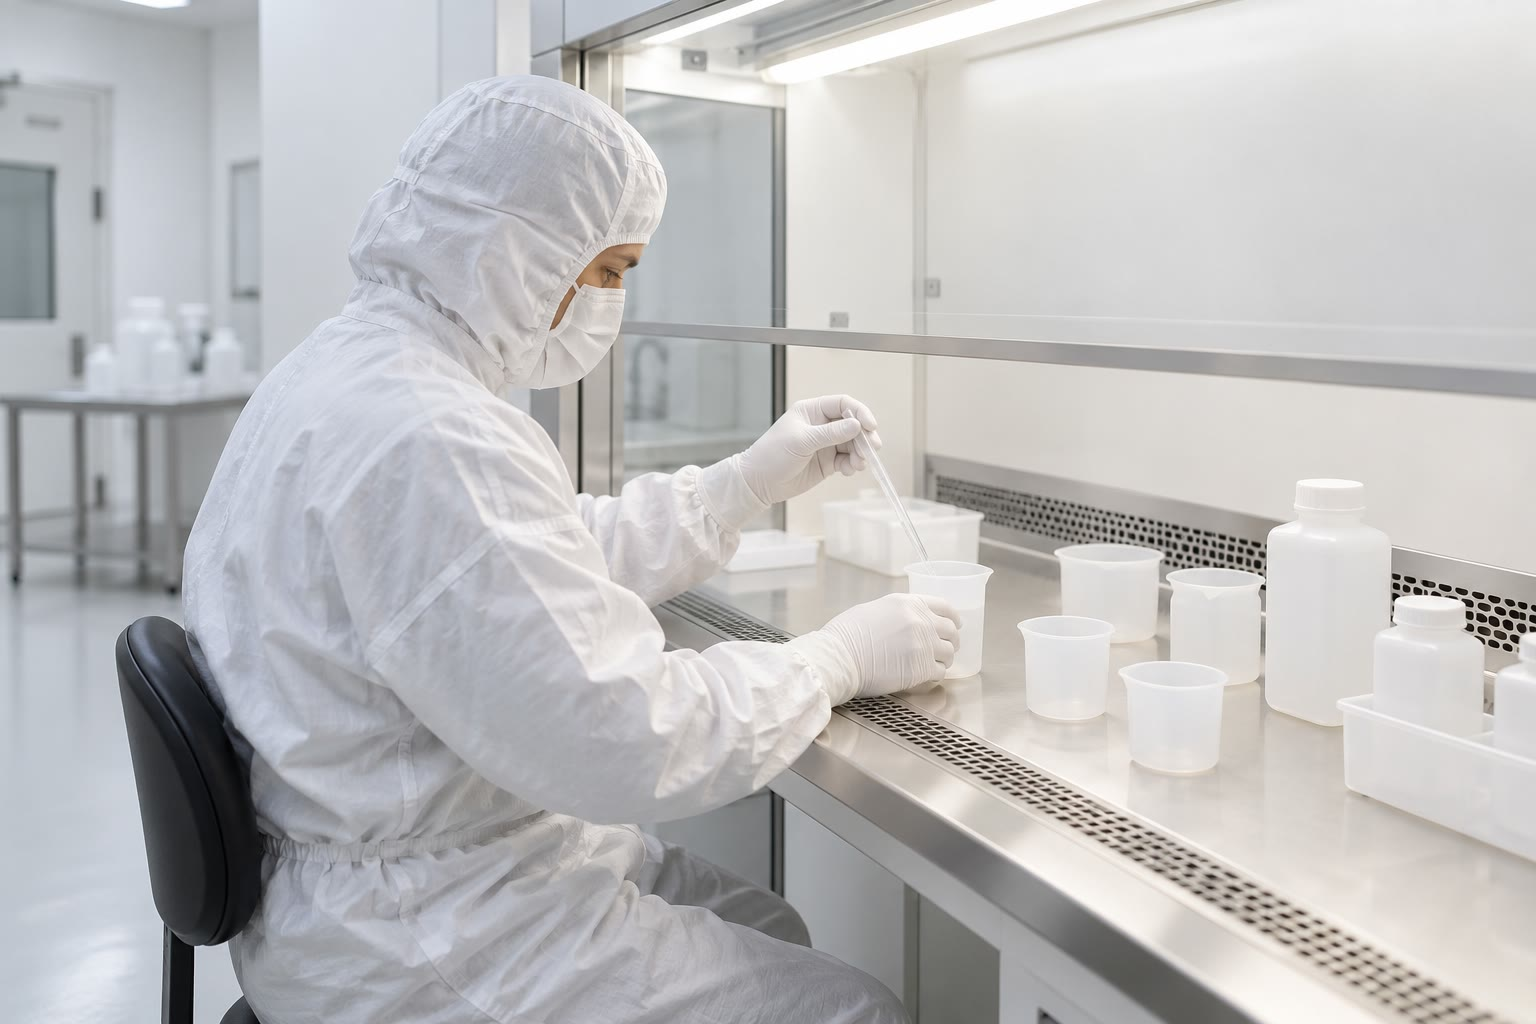
\includegraphics[width=\linewidth]{images/book4/ai/b2-clean-lab.jpg}

\smallskip
{\footnotesize Un technicien en combinaison de salle blanche au poste à flux laminaire
d'un laboratoire propre de géochimie (Illustration générée par IA.)\par}
\end{minipage}
\end{inthelab}
% ledger: usgs:bhvo2-trace, usgs:bhvo2-origin

\section{Exercices}

\begin{exercise}[$\star$]\label{exo:b2:elements-in-the-earth:1}
Le basalte BHVO-2 contient 0.5130 pour cent de \ce{K2O} et 2.731 pour
cent de \ce{TiO2} en masse. Avec les masses atomiques K 39.10, Ti 47.87
et O 16.00, calculer ses teneurs en potassium et en titane en ppm.
\end{exercise}

\begin{exercise}[$\star$]\label{exo:b2:elements-in-the-earth:2}
Dans la \omterm{def:b2:elements-in-the-earth:bse}{Terre silicatée globale}, les rapports $(X/\mathrm{Mg})$ divisés
par les rapports CI valent 1.16 pour l'aluminium, 0.22 pour le sodium, 0.077
pour le nickel et 0.0029 pour l'iridium. Les \omterm{def:b2:planet-formation-meteorites:condensation}{températures de condensation}
de ces éléments sont 1653, 958, 1353 et \qty{1603}{K}. Donner la classe
de Goldschmidt de chaque élément et expliquer chaque appauvrissement.
\end{exercise}

\begin{exercise}[$\star$]\label{exo:b2:elements-in-the-earth:3}
La croûte continentale supérieure contient \qty{31}{ppm} de lanthane
et \qty{2.0}{ppm} d'ytterbium~; les \omterm{def:b2:elements-in-the-earth:ci}{chondrites CI}, 0.232 et
\qty{0.163}{ppm}. Calculer les valeurs normalisées aux \omterm{def:b2:planet-formation-meteorites:chondrule}{chondrites} et
$(\mathrm{La}/\mathrm{Yb})_N$. Que dit ce rapport de la croûte~?
\end{exercise}

\begin{exercise}[$\star$]\label{exo:b2:elements-in-the-earth:4}
La croûte continentale supérieure contient 4.7, 1.0 et \qty{4.0}{ppm} de samarium,
d'europium et de gadolinium~; les \omterm{def:b2:elements-in-the-earth:ci}{chondrites CI}, 0.145, 0.0546 et \qty{0.198}{ppm}.
Calculer $\mathrm{Eu}/\mathrm{Eu}^*$. Quel minéral explique le résultat~?
\end{exercise}

\begin{exercise}[$\star\star$]\label{exo:b2:elements-in-the-earth:5}
Une pyroxénite à grenat est formée de 65 pour cent de clinopyroxène, 18 pour
cent de grenat et 17 pour cent d'olivine, d'orthopyroxène et de spinelle. Les
coefficients de partage du lanthane sont 0.058, 0.001 et 0.001, ceux du lutécium
0.53, 5.8 et 0.18. Calculer les coefficients globaux. Quel élément est compatible
dans la roche~? Quel minéral porte l'essentiel du lutécium de la roche~?
\end{exercise}

\begin{exercise}[$\star\star$]\label{exo:b2:elements-in-the-earth:6}
La \omterm{def:b2:elements-in-the-earth:bse}{Terre silicatée globale} contient 22.8 pour cent de magnésium, \qty{2670}{ppm}
de sodium et \qty{1960}{ppm} de nickel~; les \omterm{def:b2:elements-in-the-earth:ci}{chondrites CI}, 9.587 pour cent,
\qty{5010}{ppm} et \qty{10640}{ppm}. Calculer les rapports normalisés au magnésium
par rapport aux CI pour le sodium et le nickel. Ces deux éléments se condensent
vers \qty{1000}{K} ou au-dessus~; pourquoi le nickel est-il le plus appauvri~?
\end{exercise}

\begin{exercise}[$\star\star$]\label{exo:b2:elements-in-the-earth:7}
Un clinopyroxène cristallise à partir d'un liquide de la composition du MORB moyen,
de \qty{5.21}{ppm} de lanthane et de \qty{0.53}{ppm} de lutécium. Ses coefficients de
partage valent 0.058 pour le lanthane et 0.53 pour le lutécium. Calculer ses teneurs
en lanthane et en lutécium, ainsi que le rapport $(\mathrm{La}/\mathrm{Lu})_N$
dans le cristal par rapport à celui du liquide (CI~: La 0.232, Lu \qty{0.0237}{ppm}).
\end{exercise}

\begin{exercise}[$\star\star$]\label{exo:b2:elements-in-the-earth:8}
Normalisé au \omterm{def:b2:elements-in-the-earth:bse}{manteau primitif} (Nb \qty{0.658}{ppm}, La \qty{0.648}{ppm}), calculer
$(\mathrm{Nb}/\mathrm{La})_N$ pour la croûte continentale supérieure (Nb 12,
La \qty{31}{ppm}), le basalte hawaïen (18.10, \qty{15.20}{ppm}) et le MORB moyen
(5.24, \qty{5.21}{ppm}). Lequel porte la signature des zones de subduction~?
\end{exercise}

\begin{exercise}[$\star\star$]\label{exo:b2:elements-in-the-earth:9}
Le potassium et l'uranium sont tous deux très incompatibles. Calculer le rapport
massique K/U dans le \omterm{def:b2:elements-in-the-earth:bse}{manteau primitif} (K \qty{240}{ppm}, U \qty{0.0203}{ppm}), dans
le MORB moyen (\qty{0.160}{\percent} \ce{K2O}, U \qty{0.119}{ppm}) et dans la croûte
continentale supérieure (\qty{2.80}{\percent} \ce{K2O}, U \qty{2.7}{ppm}), en
utilisant $\mathrm{K}/\ce{K2O} = 0.830$ en masse. Que signifie la quasi-constance de
ce rapport, et pourquoi K/U est-il utile pour estimer le potassium d'une planète~?
\end{exercise}

\begin{exercise}[$\star\star\star$]\label{exo:b2:elements-in-the-earth:10}
Une faible quantité de liquide est en équilibre avec la pyroxénite à grenat
de l'exercice 5. Montrer que, pour deux éléments, le rapport
$(C_1/C_2)_{\mathrm{melt}}/(C_1/C_2)_{\mathrm{rock}}$ est égal à $\bar D_2/\bar D_1$.
Le calculer pour le lanthane et le lutécium, et expliquer pourquoi les
liquides issus d'un manteau à grenat ont des motifs de \omterm{def:b2:elements-in-the-earth:ree}{terres rares} abrupts.
\end{exercise}

\begin{exercise}[$\star\star\star$]\label{exo:b2:elements-in-the-earth:11}
Un MORB moyen (Th \qty{0.404}{ppm}, Nb \qty{5.24}{ppm}) assimile de la croûte
continentale supérieure (Th \qty{10.5}{ppm}, Nb \qty{12}{ppm})~: une fraction massique
$f$ de croûte se mélange à $1-f$ de basalte. Montrer que les concentrations du
mélange sont linéaires en $f$ mais que son rapport Th/Nb ne l'est pas. Trouver
la valeur de $f$ pour laquelle Th/Nb atteint 0.2, puis le rapport pour $f = 0.1$.
\end{exercise}

\begin{exercise}[$\star\star\star$]\label{exo:b2:elements-in-the-earth:12}
Retirer de l'eau, du carbone ou un noyau métallique ne contenant ni aluminium
ni magnésium ne modifie pas le rapport Al/Mg du reste~: le démontrer.
Dans la \omterm{def:b2:elements-in-the-earth:bse}{Terre silicatée globale}, $(\mathrm{Al}/\mathrm{Mg})$ vaut 1.16
fois la valeur CI. Si la Terre avait conservé tout son aluminium, quelle
fraction de son magnésium chondritique manquerait-il à la Terre silicatée~?
Avec le rapport du silicium normalisé au magnésium, 0.83, quelle
fraction de son silicium chondritique manquerait-il dans la même hypothèse~?
\end{exercise}

\section{Problème~: peser le noyau avec une chondrite}

\begin{problem}[{Problème du week-end --- reconstruire la Terre globale à partir des
chondrites CI, du manteau et du noyau, et peser le noyau}]
\label{pb:b2:elements-in-the-earth:1}
Une géochimiste planétaire veut peser le noyau de la Terre sans sismologie,
à partir de la seule chimie. Elle prend les \omterm{def:b2:elements-in-the-earth:ci}{chondrites CI} comme
matière de départ (Mg \qty{95870}{ppm}, Al 8500, Si \num{106500}, Fe
\num{182800}, Ni \qty{10640}{ppm}), le \omterm{def:b2:elements-in-the-earth:bse}{manteau primitif} pour la Terre
silicatée (MgO 37.8, FeO 8.05, NiO 0.25 pour cent~; Mg 22.8, Si 21.0
pour cent), et un noyau modèle de 85.5 pour cent de Fe, 5.2 pour cent
de Ni et 6.0 pour cent de Si. Masses atomiques~: Mg 24.31, Si 28.09,
Fe 55.85, Ni 58.69, O 16.00. Masse de la Terre \qty{5.972e24}{kg}.

\medskip\noindent\textbf{Partie I --- Le point de départ chondritique.}
\begin{enumerate}
\item Calculer les rapports massiques Fe/Mg, Ni/Mg, Si/Mg et Al/Mg des \omterm{def:b2:elements-in-the-earth:ci}{chondrites CI}.
\item Convertir Fe/Si en rapport atomique. La spectroscopie de la photosphère solaire donne 0.81 atome de fer
pour un atome de silicium~: la comparaison est-elle raisonnable~?
\item Les \omterm{def:b2:elements-in-the-earth:ci}{chondrites CI} contiennent 2.1 pour cent d'hydrogène et 3.5 pour cent de carbone,
liés dans des minéraux hydratés et des composés organiques que la Terre n'a pas conservés.
Pourquoi les rapports de la question 1 n'ont-ils pas besoin d'être corrigés de cette perte~?
\item Pourquoi le magnésium est-il un élément de référence adapté au problème du noyau,
et pourquoi le fer ne pourrait-il pas servir~?
\item Le nickel, le magnésium, le fer et le silicium se condensent à moins de \qty{50}{K} les uns des autres
(1353, 1336, 1334 et \qty{1310}{K}). Pourquoi cela soutient-il l'hypothèse que la Terre globale a conservé
leurs rapports chondritiques~? Quel rapport de la question 1 s'écarte de ce groupe, et que dit le chapitre
à ce sujet~?
\end{enumerate}

\noindent\textbf{Partie II --- La Terre silicatée.}
\begin{enumerate}[resume]
\item Convertir le FeO et le NiO du \omterm{def:b2:elements-in-the-earth:bse}{manteau primitif} en Fe et en Ni.
\item Calculer Fe/Mg et Ni/Mg dans la Terre silicatée.
\item Quelle fraction du Fe et du Ni chondritiques manque à la Terre silicatée,
à magnésium constant~?
\item Le même calcul pour l'iridium (\omterm{def:b2:elements-in-the-earth:bse}{manteau primitif} \qty{3.2}{ppb}, CI
\qty{0.470}{ppm}) donne une fraction manquante de 99.7 pour cent. Pourquoi est-elle plus grande
que pour le nickel, et celle du nickel plus grande que pour le fer~?
\item Où se trouve le fer dans la Terre silicatée, et pourquoi tout ce fer n'est-il pas passé
dans le noyau~?
\end{enumerate}

\noindent\textbf{Partie III --- Peser le noyau.}
\begin{enumerate}[resume]
\item Écrire le bilan du fer de la Terre avec la fraction massique $x$ du noyau, et
démontrer la \cref{prop:b2:elements-in-the-earth:core}.
\item Calculer $y = x/(1-x)$ et $x$ à partir du fer.
\item Faire de même à partir du nickel.
\item Les deux estimations ne concordent pas exactement. Les combiner par moindres carrés~:
minimiser $\sum (a_iy - b_i)^2$, où $a_i y = b_i$ sont les deux équations des
questions 12 et 13, et donner le meilleur $y$ et le meilleur $x$.
\item Pourquoi la valeur des moindres carrés est-elle si proche de l'estimation fondée sur le fer~?
\item À partir des deux équations, calculer le rapport Fe/Ni du noyau qui rendrait les deux
exactes. Comparer avec le noyau modèle.
\item Donner la masse du noyau.
\end{enumerate}

\noindent\textbf{Partie IV --- Vérifications et conséquences.}
\begin{enumerate}[resume]
\item La sismologie donne un noyau de 32.5 pour cent de la masse de la Terre. De combien
pour cent l'estimation chimique diffère-t-elle~?
\item Avec un noyau de 32.5 pour cent, quelle quantité de fer le noyau devrait-il contenir
pour fermer le bilan du fer~? Cela est-il compatible avec un noyau contenant 10 pour cent
d'éléments légers~?
\item Le noyau modèle contient 9.3 pour cent d'éléments autres que le Fe et le Ni. Quels
éléments légers sont candidats, et quelle preuve du chapitre soutient le silicium~?
\item Calculer, avec le $y$ de la question 14, la teneur en silicium du noyau qui rendrait
chondritique le rapport Si/Mg de la Terre globale.
\item Comparer avec les 6 pour cent du modèle. Proposer une raison, tirée du chapitre
précédent, pour laquelle une partie du silicium pourrait manquer totalement à la Terre.
\item Le noyau modèle contient \qty{0.5}{ppm} d'or, le \omterm{def:b2:elements-in-the-earth:bse}{manteau primitif}
\qty{1}{ppb}. Avec un noyau de 32.5 pour cent, quelle fraction de l'or terrestre se trouve
dans le noyau~?
\item Énoncer la fraction massique du noyau de la Terre obtenue à partir de la seule chimie,
le nombre clé de ce problème.
\end{enumerate}
\end{problem}
% ledger: lodders:ci-table, lodders:ci-h-photo, ms95:pm-oxides, ms95:pm-trace, mcd03:core, earth:mass, badro:core, lodders:tc-table
